 
\chapter{REFERENCIAL TEÓRICO}
\vspace{-6mm}

\section{COMPUTAÇÃO ORIENTADA A SERVIÇO}
\vspace{-6mm}


As empresas precisam estar preparadas para responder rápidamente e
eficientemente a mudanças impostas por novas regulações, por aumento de
competição ou ainda para usufruir de novas oportunidades. No contexto atual, em que as
informações fluem de modo extremamente veloz, o tempo disperdiçado pelas organizações para se
adaptar a um novo cenário tem um preço elevado, gerando expressiva perda de
receita e, em determinados casos, podendo causar a falência.

No campo das instituições governamentais, a eficiência na condução das ações do
Estado impõem que a estrutura de troca de informações entre os mais variados
entes seja continuamente adaptável, mutuamente integrada. Pode-se tomar como
exemplo a edição de nova lei que implique alteração no cálculo do tempo de
serviço para aposentadoria. A nova fórmula deve se propagar para ser
aplicada em várias instituições que compõem a máquina pública.

Nessas situações, os sistemas de informação das organizações devem possibilitar
que a dinâmica de adaptação ocorra sem demora, sob pena de, em vez de serem
ferramentais para apoiar continuamente os processos de negócio, se tornem
entrave para a ágil incorporação dos novos processos. Por outro lado, a nova
configuração deve se manter integra e funcional com o cenário de Tecnologia da
Informação -- TI -- existente, normalmente complexo.

A eficiência na integração entre as soluções de TI é determinante para que se
consiga alterar uma parte sem comprometer todo o ecossistema. A integração
possibilita a combinação de eficiência e flexibilidade de recursos para otimizar
a operação através e além dos limites de uma organização, proporcionando maior
interoperabilidade \cite{papazoglou2008service}.

A computação orientada a serviços -- SOC -- endereça essas necessidades em uma
plataforma que aumenta a flexibilidade e melhora o alinhamento com o negócio, a
fim de reagir rapidamente a mudanças nos requisitos de negócio. Para obter esses
benefícios, contudo, os serviços devem cumprir com determinados quesitos, que
incluem alta autonomia ou baixo acoplamento \cite{erl2008soa}. Assim, o paradigma de SOC
está voltado para o projeto de soluções preparadas para constantes mudanças,
substituindo-se continuamente pequenas peças -- os serviços -- por outras
atualizadas.

Portando, o objetivo da SOC é conceber um estilo de projeto, tecnologia e
processos que permitam às empresas desenvolver, interconectar e manter suas
aplicações e serviços corporativos com eficiência e baixo custo. Embora esses
objetivos não sejam novos, SOC procura superar os esforços prévios como
programação modular, reuso de código e técnicas de desenvolvimento orientadas a
objetos \cite{papazoglou2007serviceApprTechRechIss}.

As vertentes mais visionárias da computação orientada a serviços prevêem, em seu
estado da arte, uma coordenação de serviços cooperantes por todo o mundo, onde
os componentes possam ser conectados facilmente em uma rede de serviços pouquíssimo acoplados e, assim, criar
processos de negócio dinâmicos e aplicações ágeis entre organizações e plataformas de
computação \cite{leymann2005combining}.


\subsection{Terminologia}
\vspace{-6mm}

\begin{description}
\item [Computação orientada a serviço] é um termo \textit{guarda-chuva} para
descrever uma nova geração de computação distribuída. Desse modo, é um conceito
que engloba vários pontos, como paradigmas e princípios de projeto, catálogo de
padrões de projeto, padronização de linguagem, modelo arquitetural específico, e
conceitos correlacionados, tecnologias e plataformas.
A computação orientada a serviços é baseada em modelos anteriores de computação
distribuída e os extendem com novas camadas de projeto, aspectos de governança,
e uma grande gama de tecnologias de implementações especializadas, em grande
parte baseadas em \ws{} \cite{erl2009web}.

\item [Orientação a serviço] é um paradígma de projeto cuja intenção é a criação
de unidades lógicas moldadas individualmente para poderem ser utilizadas
conjutamente e repetidamente, atendendo assim a objetivos e
funções específicos associados com SOA e computação orientada a serviço.

A lógica concebida de acordo com orientação a serviço pode ser designada de
\textbf{orientada a serviço}, e as unidades da lógica orientada a serviço são
referenciadas como \textbf{serviços}. Como um paradigma de computação
distribuída, a orientação a serviço pode ser comparada a orientação a objetos,
de onde advém várias de suas raízes, além da influência de
\textit{Interface Description Languages} -- EAI,
\textit{Business Process Modeling} -- BPM e \ws \cite{erl2009web}.

A orientação a serviços é composta principalmente de oito princípios de projeto
(os quais serão descritos na subseção \ref{PrincipiosSOA}).

\item [Arquitetura orientada a serviço - SOA] representa um modelo arquitetural
cujo objetivo é elevar a agilidade e a redução de custos e ao mesmo tempo
reduzir o peso da Tecnologia da Informação (TI) para a organização. Isso é feito
colocando o serviço como elemento central da representação lógica da solução \cite{erl2009web}.

Como uma arquitetura tecnológica, uma implementação SOA consiste da combinação
de tecnologias, produtos, APIs, extensões da infraestrutura, etc. A implantação
concreta de uma arquitetura orientada a serviço é única para cada organização,
entretanto é caracterizada pela introdução de tecnologias e plataformas que
suportam a criação, execução e evolução de soluções orientadas a serviços. O
resultado é a formação de um ambiente projetado para produzir soluções alinhadas
aos princípios de projeto de orientação a serviço.

Segundo Thomas Erl \cite{erl2009web}, o termo arquitetura orientada a serviço --
SOA -- vem sendo amplamente utilizado na mídia e nos produtos de divulgação de
fabricantes e se tornado quase que sinônimo de computação orientada a
serviço -- SOC.

\item [Serviço] é a unidade da solução no qual foi aplicada a orientação a
serviço. É a aplicação dos princípios de projeto de orientação a
serviço que distigue uma unidade de lógica como um serviço comparada a outras
unidades de serviços que podem existir isoladamente como um objeto ou
componente \cite{erl2009web}.

Após a modelagem conceitual do serviço, os estágios de projeto e desenvolvimento
produzem um serviço que é um programa de \textit{software} independente com
características específicas para suportar a realização dos objetivos associados
a computação orientada a serviço.

Cada serviço possui um contexto funcional distinto e é composto de uma lista
de capacidades relacionadas a esse contexto. Então um serviço pode ser
considerado um conjunto de capacidades descritas em seu contrato.


\item [Contrato de serviço] é o conjunto de documentos que expressam as
meta-informações do serviço, sendo a parte que descreve a
sua interface técnica, a mais fundamental. Esses documentos compõem o contrato
técnico do serviço, cuja essência é estabelecer uma API com as funcionalidades providas pelo serviço por meio de
suas capacidades \cite{erl2009web}.

Os serviços implementados como \ws{} SOAP normalmente são descritos em
arquivos \ws{} \textit{Description Language} -- WSDL, \textit{XML
schemas} and políticas (\textit{WS-policy}). Já os serviços implementados como \ws{} REST não
possuem uma linguagem padrão para especificação de contratos. Já foram propostas
algumas alternativas como WADL \cite{hadley2006web}, Swagger \cite{swaggerSite},
e \neoidl{} \cite{lima2015neoidl}.

O contrato de serviço também pode ser composto de documentos de leitura humana,
como os que descrevem níveis de serviços (\textit{SLA}), comportamentos e
limitações. Muitas dessas características também podem ser descritas em
linguagens formais (para processamento computacional).

No contexto de orientação a serviço, o projeto do contrato do serviço é de suma
importância de tal forma que o princípio de projeto contrato de serviço
padronizado dedica-se exclusivamente ao cuidado com contratos de serviços
uniformes e de qualidade \cite{erl2009web}.

\end{description}


\subsection{Objetivos, benefícios e características}
\vspace{-6mm}

De modo diferente de arquiteturas convencionais, ditas monolíticas, em que os
sistemas são concebidos agregando continuamente funcionalidades a um mesmo pacote de
\textit{software}, a arquitetura orientada a serviço prega o projeto de pequenas
aplicações distribuídas que podem ser consumidas tanto por usuários finais como
por outros serviços \cite{papazoglou2007serviceApprTechRechIss}. 

A unidade lógica da arquitetura orientada a serviços é exatamente o serviço.
Serviços são pequenos \textit{softwares} que provêem funcionalidades específicas
para serem reutilizadas em várias aplicações. Cada serviço é uma entidade isolada com
dependências limitadas de outros recursos compartilhados
\cite{serrano2014service}. Assim, é formada uma abstração entre os fornecedores
e consumidores dos serviços, por meio de baixo acoplamento, e promovendo a
flexibilidade de mudanças de implementação sem impacto aos consumidores.

A arquitetura SOC busca atingir um conjunto de objetivos e benefícios
\cite{erl2008soaDesigPatterns}:
\begin{enumerate}[(a)] 
  \item Ampliar a interoperabilidade intrínseca, de modo a se ter uma rápida
  resposta a mudanças de requisitos de negócio por meio da efetiva
  reconfiguração das composições de serviços;
  \item Ampliar a federação da solução, permitindo que os serviços possam ser
  evoluídos e governados individualmente, a partir da uniformização de
  contratos;
  \item Ampliar a diversificação de fornecedores, fazendo com que se possa
  evoluir a arquitetura em conjunto com o negócio, sem ficar restrito a
  características de derminados fornecedores;
  \item Ampliar o alinhamento entre a tecnologia e o negócio, especializando-se
  alguns serviços ao contexto do negócio e possibilitando sua evolução;
  \item Ampliar o retorno sobre investimento, pois muitos serviços podem
  ser rearranjados em novas composições sem que se tenha que se construir
  grandes soluções de custo elevado;
  \item Ampliar a agilidade, remontando as composições por reduzido esforço,
  beneficiando-se do reuso e interoperabilidade nativas dos serviços;
  \item Reduzir o custo de TI, como resultado de todos os benefícios acima
  citados.
\end{enumerate}

Para possibilitar que esses benefícios sejam atingidos, quatro características
são observadas em qualquer plataforma SOA. A primeira é o direcionamento
efetivo ao negócio, levando-se em conta os objetivos estratégicos de negócio na
concepção do projeto arquitetural. Se isso não ocorrer, é inevitável que o
desalinhamento com os requisitos de negócio cheguem a níveis muito elevados
bem rapidamente \cite{erl2008soaDesigPatterns}.

A segunda característica é a independência de fabricante. O projeto arquitetural
que considera apenas um fabricante específico levará inadvertidamente a
implantação dependente de características proprietárias. Essa dependência também
reduzirá a agilidade na reação às mudanças e tornará a arquitetura inefetiva. A
arquitetura orientada a serviço deve fazer uso de tecnologias providas pelos
fornecedores, sem, no entanto, se tornar dependente dela, por meio de APIs e
protocolos padrões de mercado.

Outra característica da aplicação da plataforma SOA é os serviços serem
considerados recursos corporativos, ou seja, da empresa como um todo. Serviços
desenvolvidos para atender um único objetivo perdem esta característica e se
assemelham a soluções de propósito específico, tal como soluções monolíticas. O
modelo arquitetural deve se guiar pela premissa de que os serviços serão
compartilhados por várias áreas da empresa ou farão parte de soluções maiores,
como serviços compatilhados.

A capacidade de composição é a quarta característica. Os serviços devem ser
projetados não somente para serem reusados, mas também para possuir
flexibilidade em serem compostos em diferentes estruturas de variadas
soluções. Confiabilidade, escalabilidade, troca de dados em tempo de execução
com integridade são pontos chave para essa característica.



\subsection{Princípios SOA}
\label{PrincipiosSOA} 
\vspace{-6mm}

O paradigma de orientação a serviço é estruturado em oito princípios
fundamentais \cite{erl2009web}, ilustrados na Figura \ref{Fig:PrincipiosSoa}. São eles que
caraterizam a abordagem SOA e a sua aplicação faz com que um serviço se diferencie de um componente ou de
um módulo. Os contratos de serviços permeiam a maior parte destes princípios.

\begin{figure}[!htb]
\centering
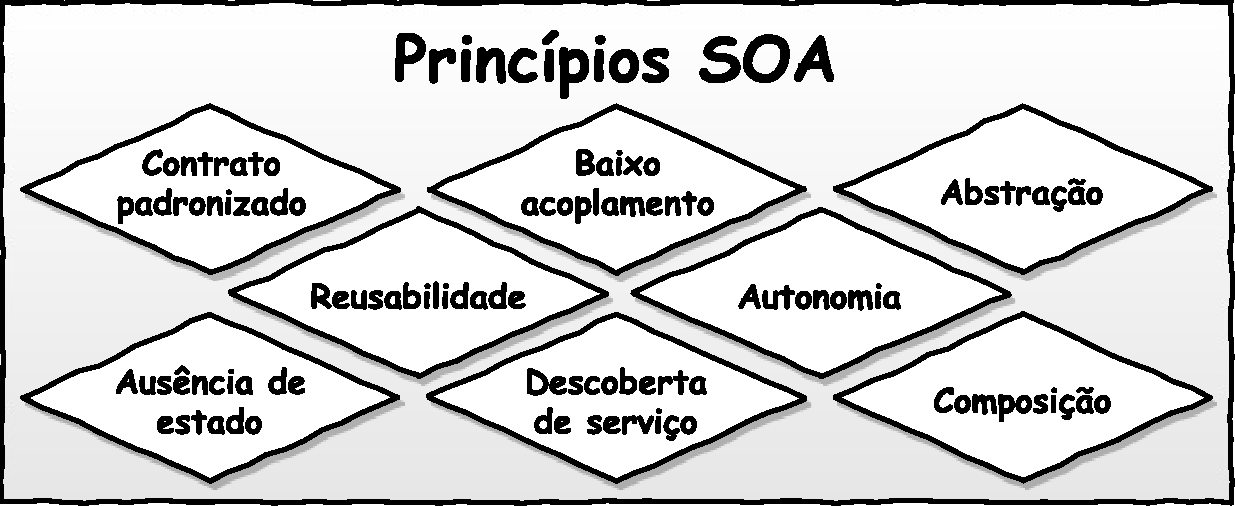
\includegraphics[width=100mm,trim = 0mm 0mm 0mm 
0mm,clip]{img/PrincipiosSOA.pdf}
\caption{Oito princípios da arquitetura orientada a serviços \cite{erl2009web}}
\label{Fig:PrincipiosSoa}
\end{figure}

\begin{description}
\item[Contrato padronizado] - \textbf{Serviços dentro de um mesmo inventário
estão em conformidade com os mesmos padrões de contrato de serviço}.
Os contratos de serviços são elementos fundamentais na arquitetura orientada a
serviço, pois é por meio deles que os serviços interagem uns com os outros e com
potenciais consumidores. Este princípio tem como foco principal o contrato de
serviço e seus requisitos. O padrão de projeto \CtFirst{} é uma
consequência direta deste princípio \cite{erl2009web}.

\item[Baixo acomplamento] - \textbf{Os contratos de serviços impõem aos
consumidores do serviço requisitos de baixo acoplamento e são, os próprios
contratos, desacoplados do seu ambiente}. 
Este princípio também possui forte relação com o contratos de serviço, pois a
forma como o contrato é projetado e posicionado na arquitetura é que gerará o
benefício do baixo acoplamento. O projeto deve garantir que o contrato
possua tão somente as informações necessárias para possibilitar a compreensão e
o consumo do serviço, bem como não possuir outras características que gerem
acoplamento.

São considerados negativos, e que devem ser evitados, os acoplamentos  
\begin{enumerate}[(a)] 
\item do contrato com as funcionalidades que ele suporta, agregando ao
contrato características específicas dos processos que o serviço atende;
\item do contrato com a sua implementação, invertendo a estratégia de conceber
primeiramente o contrato;
\item do contrato com a sua lógica interna, expondo aos consumidores
características que levem os consumidores a inadivertidamente aumentarem o
acoplamento;
\item do contrato com a tecnologia do serviço, causando impactos indesejáveis em
caso de substituição de tecnologia.
\end{enumerate}

Por outro lado, há um tipo de acoplamento positivo que é o que gera dependência
da lógica em relação ao contrato \cite{erl2009web}. Ou seja, idealmente a
implementação do serviço deve ser derivada do contrato, pondendo se ter inclusive a geração de código a
partir do contrato.


\item[Abstração] - \textbf{Os contratos de serviços devem conter apenas
informações essenciais e as informações sobre os serviços são limitadas àquelas
publicadas em seus contratos}. O contrato é a forma oficial a partir da qual o
consumidor do serviço faz seu projeto e tudo o que está além do contrato deve
ser desconhecido por ele. Por um lado este princípio busca a ocultação
controlada de informações. Por outro, visa a simplificação de informações do
contrato de modo a assegurar que apenas informações essenciais estão
disponíveis.


\item[Reusabilidade]- \textbf{Serviços contém e expressam lógica agnóstica e
podem ser disponibilizados como recursos reutilizáveis}. Este princípio
contribui para se entender o serviço como um produto e seu contrato com uma API
genérica para potenciais consumidores. Essa abordagem aplicada ao projeto dos
serviços leva a desenhá-lo com lógicas não dependentes de processos de negócio
específicos, de modo a torná-los reutilizáveis em vários processos.

\item[Autonomia]- \textbf{Serviços exercem um elevado nível de controle sobre
o seu ambiente em tempo de execução}. O controle do ambiente não está ligado a
dependência do serviço à sua plataforma em termos de projeto, mas sim ao aumento
da confiabilidade sobre a execução e redução da dependência dos recursos
sobre os quais não se tem controle.
O que se busca é a previsibilidade sobre o comportamento do serviço.

\item[Ausência de estado] - \textbf{Serviços reduzem o consumo de recursos
restringindo a gestão de estado das informações apenas a quando for necessário}.
Este princípio visa reduzir ou mesmo remover a sobrecarga gerada pelo
gerenciamento do estado de cada operação, aumentando a escalabilidade da
plataforma de arquitetura orientação a serviço como um todo. Na composição do
serviço, o serviço deve armazenar apenas os dados necessários para completar o
processamento, enquanto se aguarda o processamento do serviço acionado.

\item[Descoberta de serviço] - \textbf{Serviços devem conter metadados por meio
dos quais os serviços possam ser descobertos e interpretados}. Tornar cada
serviço de fácil descoberta e interpreção pelas equipes de projeto é o foco
deste princípio. Os próprios contratos de serviço devem ser projetados para
incorporar informações que auxiliem na sua descoberta.

\item[Composição] - \textbf{Serviços são participantes efetivos de composição,
independentemente do tamanho ou complexidade da composição}. O princípio da
composição faz com que os projetos de serviços sejam projetados para
possibilitar que eles se tornem participantes de composições. Deve-se levar em
conta, entretanto, os outros princípios no planejamento de uma nova composição,
considerando a complexidade das composições a serem formadas.

\end{description}
 

\subsection{Contract First}
\vspace{-6mm}

O princípio do baixo acoplamento tem por objetivo principal reduzir o
acoplamento entre o cliente e o fornecedor do serviço. Há vários tipos de
acopamentos negativos, como citado na subseção \ref{PrincipiosSOA}. Porém, um
acoplamento é considerado positivo e desejável: da implementação a partir do contrato. Ou seja, a lógica
do serviço deve corresponder ao que está especificado no contrato.

Duas abordagens podem ser seguidas para se produzir esse efeito. A primeira é a
geração do contrato a partir da lógica implementada, conhecida como
\CdFirst{}. A outra propõe um sentido inverso, partindo-se do contrato
para a geração do código, chamada \CtFirst{}. A abordagem
\CtFirst{} é recomendada para a arquitetura orientada a serviço
\cite{erl2009web}.

Embora muitas vezes preferível pelo desenvolvedor, a desvantagem do uso
\CdFirst{} está no elevado impacto que alterações na implementação causam ao
contrato, fazendo com que os clientes dos serviços sejam também afetados.
Reduz-se a flexibilidade e extensibilidade, de modo que o reuso é prejudicado. Ainda,
eleva-se o risco de os serviços serem projetados para aplicações específicas e
não voltados para reuso e composição \cite{karthikeyancontract}.

A abordagem \CtFirst{} preocupa-se principalmente com a clareza, completude e
estabilidade do contrato para os clientes dos serviços. Toda a
estrutura da informação é definida sem a preocupação sobre restrições ou
características das implementações subjacentes. Do mesmo modo, as
capacidades são definidas para atenderem a funcionalidades a que se destinam,
porém com a preocupação em se promover estabilidade e reuso.

As principais vantagens do \CtFirst{} estão no baixo acoplamento do contrato em
relação a sua implementação, na possibilidade de reuso de esquemas de dados (XML
ou JSON Schema), na simplificação do versionamento e na facilidade de manutenção
\cite{karthikeyancontract}. A desvantagem está justamente na complexidade de
escrita do contrato. Porém, várias ferramentas já foram e vem sendo
desenvolvidas para facilitar essa tarefa.


\section{WEB SERVICES}
\vspace{-6mm}

\ws{} são aplicações modulares e autocontidas que podem ser publicadas,
localizadas a acessadas pela \textit{Web} \cite{alonso2004web}. A diferença
entre o \ws{} e a aplicação \textit{Web} propriamente dita é que o primeiro se
preocupa apenas com o dado gravado ou fornecido, deixando para o cliente a atribuição de apresentar a
informação \cite{serrano2014service}.

A necessidade das organizações de integrar suas soluções, seja
entre os sistemas internos ou entre esses e sistemas de outras empresas
\cite{rao2004survey}, não é recente. Essa é uma das principais motivações do uso
de \ws{}, por possibilitar que soluções construídas com tecnologias distintas
possam trocar informações por meio da \textit{Web}. Nesse contexto, as arquiteturas
orientadas a serviço fazem amplo uso de \ws{} como meio para disponibilização de serviços.

Há dois tipos de \ws{}: baseados em SOAP e baseados em REST. Os mais diversos
tipos de aplicações podem ser concebidas utilizando \wss{} SOAP ou REST,
situação também aplicável a serviços.
Originalmente os serviços utilizaram \ws{} SOAP, trafegando as informações em
uma mensagem codificada em um formato de troca de dados (XML), por meio do
protocolo SOAP (seção \ref{secaoSOAP}). Entretanto, a adoção de \ws{} REST
(seção \ref{secaoREST}) tem ganhado popularidade \cite{mumbaikar2013web}.

\subsection{SOAP (W3C) }
\label{secaoSOAP}
\vspace{-6mm}

SOAP -- \textit{Simple Object Access Protocol} -- é um protocolo padrão W3C que
provê uma definição de como trocar informações estruturadas, por meio de XML, entre
as partes de ambientes descentralizados ou distribuídos \cite{WSDLSite}. SOAP
é um protocolo mais antigo que REST, e foi desenvolvido para troca de informações
pela Internet se utilizando de protocolos como HTTP, SMTP, FTP, sendo o primeiro
o mais comumente utilizado.

Por ser anterior, SOAP é o padrão de \ws{} mais comumente utilizado pela
indústria.
Algumas pessoas chegam a tratar \ws{} apenas como SOAP e WSDL
\cite{serrano2014service}. SOAP atua como um envelope que transporta a mensagem
XML, e possui vastos padrões para transformar e proteger a mensagem e a
trasmissão. 


\subsubsection{Especificação de contratos}
\vspace{-6mm}

Os contratos em SOAP são especificados no padrão WSDL -- \textit{Web Services
Description Language} -- que define uma gramática XML para descrever os serviços
como uma coleção de \textit{endpoints} capazes de atuar na troca de mensagens.
As mensagens e operações são descritas abstratamente na primeira seção do
documento. Uma segunda seção, dita concreta, estabelece o protocolo de rede e o
formato das mensagens.

Muitas organizações preferem utilizar SOAP por ele dispor de mais mecanismos de
segurança e tratamento de erros \cite{serrano2014service}. Além disso, a tipagem
de dados é mais forte em SOAP que em REST \cite{mumbaikar2013web}.


\subsection{REST (Fielding)}
\label{secaoREST}
\vspace{-6mm}

O termo REST foi criado por Roy Fielding, em sua tese de doutorado
\cite{fielding2000architectural}, para descrever um modelo arquitetural
distribuído de sistemas hipermedia. Um \ws{} REST é baseado no conceito de
recurso (que é qualquer coisa que possua uma \textit{Uniform Resource
Identifier} -- URI) que pode ter zero ou mais representações
\cite{he2003service}.

O estilo arquitetural REST é cliente-servidor, em que o cliente envia uma
requisição por um determinado recurso ao servidor e este retorna uma resposta.
Tanto a requisição como a resposta ocorrem por meio da transferência de
representações de recursos \cite{mumbaikar2013web}, que podem ser de vários
formatos, como XML e JSON \cite{serrano2014service}. Toda troca de informações
ocorre por meio do protocolo HTTP, com uma semântica específica para cada
operação:

\begin{enumerate}
\item HTTP GET é usado para obter a representação de um recurso.
\item HTTP DELETE é usado para remover a representação de um recurso.
\item HTTP POST é usado para atualizar ou criar a representação de um recurso.
\item HTTP PUT é usado para criar a representação de um recurso.
\end{enumerate}

As transações são independentes entre si e com as transações anteriores, pois o
servidor não guarda qualquer informação de sessão do cliente. Todas as
informações de estado são trafegadas nas próprias requisições, de modo que as
respostas também são independentes. Essas características tornam os \wss{} REST
simples e leves \cite{mumbaikar2013web}.

O uso de REST tem se tornado popular por conta de sua flexibilidade e
performance em comparação com SOAP, que precisa envelopar suas informações em
um pacote XML \cite{mumbaikar2013web}, de armazenamento, transmissão e
processamento onerosos.

\subsubsection{Especificação de contratos}
\vspace{-6mm}

Ao contrário de SOAP, REST não dispõe de um padrão para especificação de
contratos. Essa carência, que no início não era considerada um problema, foi se
tornando uma necessidade cada vez mais evidente a medida em que se amplia o
conjunto de \wss{} implantados. Atualmente, existem algumas linguagens com o
propósito de documentar o contrato REST.

A linguagem mais popular atualmente é \textit{Swagger} cujo projeto se iniciou
por volta de 2010 para atender a necessidade de um projeto específico, sendo posteriormente
vendida para uma grande empresa. Em janeiro de 2016, \textit{Swagger} foi doada
para o \textit{Open API Iniciative (OAI)} e denominada de \textit{Open API
Specification}. O propósito da iniciativa é tornar \textit{Swagger} padrão para
especificação de APIs com independencia de fornecedor. Apoiam o projeto grandes
empresas como Google\textsuperscript{\textregistered},
Microsoft\textsuperscript{\textregistered} e
IBM\textsuperscript{\textregistered}.

WADL (\textit{Web Application Description Language}), uma especifição baseada em
XML semelhante ao WSDL, foi projetada e proposta pela \textit{Sun
Microsystems}\textsuperscript{\textregistered} e sua última versão submetida
ao W3C em 2009. Outra linguagem proposta é a RAML\cite{RAML} -- abreviação de
\textit{RESTful API Modeling Language} -- baseada em YAML e projetada pela
MuleSoft\textsuperscript{\textregistered}. Muitos projetos \textit{open source} adotam RAML.

Todas estas linguagens possuem suporte tanto para \CdFirst{} como para
\CtFirst{} \cite{wideberg2015restful}.



%\subsubsection{Outros padrões }
%\vspace{-6mm}
%\ldots

\section{DESIGN BY CONTRACT}
\label{Design-by-Contract}
\vspace{-6mm}

\designbycontract{} \cite{meyer1992applying} - DbC - é um conceito
oriundo da orientação a objetos, no qual consumidor e fornecedor firmam entre si garantias para
o uso de métodos ou classes. De um lado o consumidor deve garantir que, antes da
chamada a um método, algumas condições sejam por ele satisfeitas.
Do outro lado o fornecedor deve garantir, se respeitadas suas exigências,
o sucesso da execução.

O mecanismo que expressa essas condições são chamados de asserções
(\textit{assertions}, em inglês). As asserções que o consumidor deve respeitar
para fazer uso da rotina são chamadas de \textbf{precondições}. As asserções que
asseguram, de parte do fornecedor, as garantias ao consumidor, são denominadas
\textbf{pós-condições}.

DbC tem o objetivo de aumentar a robustez do sistema e tem na linguagem Eiffel
\cite{meyer1988eiffel} um de seus precursores. Para os mantenedores do Eiffel, DbC é
tão importante quanto classes, objetos, herança, etc. O uso de DbC na
concepção de sistemas é uma abordagem sistemática que produz sistemas com mais
corretude.

O conceito chave de \designbycontract{} é ver a relação entre a classe e
seus clientes como uma relação formal, que expressa os direitos e as
obrigações de cada parte \cite{meyer1997object}. Se, por um lado, o
cliente tem a obrigação de respeitar as condições impostas pelo fornecedor para fazer uso do módulo, por
outro, o fornecedor deve garantir que o retorno ocorra como esperado.

As precondições vinculam o cliente, no sentido de definir as condições que
o habilitam para acionar o recurso. Corresponde a uma obrigação para o cliente e
o benefício para o fornecedor \cite{meyer1997object} de que certos
pressupostos serão sempre respeitados nas chamadas à rotina.
As pós-condições vinculam o fornecedor, de modo a definir as condições para que o retorno ocorra.
Corresponde a uma obrigação para o fornecedor e o benefício para o cliente de
que certas propriedades serão respeitadas após a chamada à rotina.

De forma indireta, \designbycontract{} estimula um cuidado maior na análise das
condições necessárias para, de forma consistente, se ter o funcionamento correto
da relação de cooperação cliente-fornecedor.
Essas condições são expressas em cada contrato, o qual especifica as obrigações
a que cada parte está condicionada e, em contra-ponto, os benefícios garantidos.

Nesse contexto, o contrato é um veículo de comunicação, por meio do qual os
clientes tomam conhecimento das condições de uso, em especial das precondições.
É fundamental que as precondições estejam acessíveis para todos os clientes
para os quais as rotinas estão disponíveis, pois, sem que isso ocorra, o cliente
corre o risco de acionar a rotina fora de suas garantias de funcionamento. 

Segundo Bertrand Meyer \cite{meyer1997object}, \designbycontract{} é um
ferramental para análise, projeto, implementação e documentação, facilitando a
construção de \textit{softwares} cuja confiabilidade é embutida, no lugar de
buscar essa característica por meio de depuração. Meyer utiliza uma expressão de
Harlan D. Mills \cite{mills1975new} para afirmar que \designbycontract{} permite
construir programas corretos e saber que eles estão corretos.

Com o uso de \designbycontract{}, cada rotina é levada a realizar o trabalho
para o qual foi projetada e fazer isso bem: com corretude, eficiência e
genericamente suficiente para ser reusada. Por outro lado, especifica de forma
clara o que a rotina não trata. Esse paradigma é coerente, pois para que a
rotina realize seu trabalho bem, é esperado que se estabeleça bem as
circunstâncias de execução.

Outra característica da aplicação de \designbycontract{} é que o recurso tem sua
lógica concentrada em efetivamente cumprir com sua função principal, deixando
para as precondições o encargo de validar as entradas de dados. Essa abordagem
é o oposto à ideia de programação defensiva, pois vai de encontro à realização
de checagens redundantes. Se os contratos são precisos e explícitos, não há
necessidade de testes redundantes \cite{meyer1992applying}.

Todos esses aspectos são fundamentais para se possibilitar o reuso eficiente de
componentes, que é o pilar da orientação a objetos e se aplica de forma análoga
à orientação a serviços. Componentes reusáveis por várias aplicações devem ser
robustos pois as consequências de falhas ou comportamentos incorretos são muito
piores que as de aplicações que atendem a único propósito
\cite{meyer1992applying}.

Há de se registrar ainda que, em orientação a objetos, existe outro tipo de
asserção além das pré e pós-condições. Em vez de cuidar das propriedades de cada
rotina individualmente, elas expressam condições globais para todas as
instâncias de uma classe \cite{meyer1997object}. Essa categoria de
asserção é denominada invariante. Uma vez que em orientação a serviço se
preconiza a ausência de estado, o conceito de invariante não é explorado neste trabalho.



\subsection{Implementações de DbC}
\label{implementDbC}

\begin{description}
\item[Eiffel] - A linguagem Eiffel foi desenvolvida em meados dos anos 80 por
Bertrand Meyer \cite{meyer1988eiffel} com o objetivo de criar ferramentas que
garantissem mais qualidade aos \textit{softwares}. A ênfase do projeto de
Eiffel foi promover reusabilidade, extensibilidade e compatibilidade.
Características que só fazem sentido se os programas forem corretos e
robustos.

Foi essa preocupação que incorporou à linguagem Eiffel o conceito de contratos.
A partir desse estilo de projeto se criou a noção de \designbycontract{},
concretizada na linguagem por meio das precondições, pós-condições e invariantes
\cite{meyer1988eiffel}. Esta abordagem influenciou outras linguagem de programação orientadas a objeto.

A figura \ref{lst:exemploEiffel} apresenta um exemplo de especificação de pré e
pós-condição na linguagem Eiffel.

\vspace{6mm}

\begin{figure}[h]
\begin{small}
\lstinputlisting[language=Eiffel,firstnumber=1]{trechos_codigo/exemploEiffel.tex}
\vspace{-.5cm}
\end{small}
\caption{Exemplo de pré e pós-condições em Eiffel}
\label{lst:exemploEiffel}
\end{figure}


\item[JML] - \textit{Java Modeling Language} é uma extensão da linguagem Java
para suporte a especificação comportamental de interfaces, ou seja, controlar o
comportamento de classes em tempo de execução. Para realizar essa função, JML
possui amplo suporte a \designbycontract{}. As asserções (precondição,
pós-condição e invariantes) são incluídas no código Java na forma de comentários
(//@ ou /*@\ldots@*/).

JML combina a praticidade de \designbycontract{} de linguagens como Eiffel com a
expressividade e formalismo de linguagens de especificação orientadas a modelo
\cite{leavens2006design}. 

A figura \ref{lst:exemploJML} apresenta um exemplo de especificação de pré e
pós-condição na linguagem de extensão JML.

\begin{figure}[h]
\begin{small}
\lstinputlisting[language=JML,firstnumber=1]{trechos_codigo/exemploJML.tex}
\vspace{-.5cm}
\end{small}
\caption{Exemplo de pré e pós-condições em JML}
\label{lst:exemploJML}
\end{figure}
 
\vspace{8mm}

\item[Spec\#] - é uma extensão da linguagem C\#, à qual agrega o suporte para
distinguir referência de objetos nulos de referência a objetos possivelmente não
nulos, especificações de pré e pós-condições e um método para gerenciar
exceções entre outros recursos \cite{barnett2004spec}.

A figura \ref{lst:exemploSpec} apresenta um exemplo de especificação de pré e
pós-condição na linguagem Spec\#.

\vspace{6mm}

\begin{figure}[h]
\begin{small}
\lstinputlisting[language=SpecSharp,firstnumber=1]{trechos_codigo/exemploSpecSharp.tex}
\vspace{-.5cm}
\end{small}
\caption{Exemplo de pré e pós-condições em Spec\#}
\label{lst:exemploSpec}
\end{figure}


\end{description}





 

